\subsection{Introduction to Anderson Localization}
% \begin{figure}[htbp]
%     \centering
%     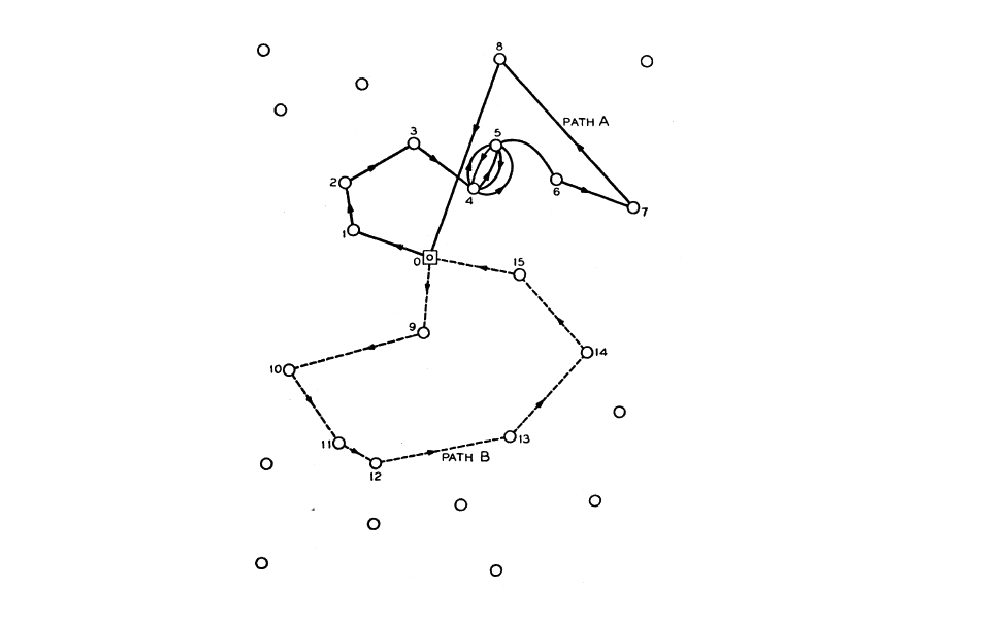
\includegraphics[width=\textwidth]{Chapter3_secs/AL1.pdf}
%     \caption{Fig.~(1) in \cite{anderson1958absence}, two kinds of scattering paths originated from lattice site 0. Path A may be large and must be summed over. Path B is a legitimate term. The potential energy at each lattice site j, $E_j$ is a random variable.}
%     \label{fig:AL1}
% \end{figure}

In the paper that introduced AL \cite{anderson1958absence}, the author studied the motion of some mobile entities in certain random lattices. It can be spins in a random field or electrons in a disordered crystal. The entities move by jumping from site to site. Starting from the most general case, the wave function of an entity can be expanded in the basis of the Wannier functions on each lattice site, 
\begin{equation}
    \hat{\psi}(\Vec{r}) = \sum_j W(\Vec{r}-\Vec{r}_j)\hat{a}_j.
\end{equation}
The Hamiltonian is
\begin{equation}
    \hat{H} = \sum_j E_j \hat{a}_j^\dag\hat{a}_j + \sum_{j<k}(V_{jk}\hat{a}_j^\dag\hat{a}_k + c.c)
\end{equation}
Here $E_j$ is the potential energy at site $j$, it is a random variable and has probability density distribution $E_j \sim \mathbb{P}(E)dE$ which is characterized by a width $W$. $V_{jk}$ is the coupling of states on site $j$ and site $k$, it can be random or non-random.

Under the following two conditions, it was proved in \cite{anderson1958absence} the wave function will be localized in a small region without diffusion. Here localization means at $t=0$, starting at site $j$, $a_j(0) = 1$, and $a_j(\infty)$ remains finite.
\begin{itemize}
    \item Low density of sites. The average coupling strength between states at different lattice sites $\langle V_{jk} \rangle < V_c$, $V_c$ is of the magnitude of $W$.
    \item $V(r)$ falls off faster than $\frac{1}{r^3}$ as $r \to \infty$.
\end{itemize}

Intuitively, the probability of diffusion from the initial site $j$ depends on the number of energy matching sites $k$ and the coupling strength between site $j$ and sites $k$. Starting from the original state at site $j$, consider the sites $k$ within the sphere of radius $r$ originated from the site $j$. As $r$ increases, the probability of finding more energy matching sites $k$ within the sphere of radius $r$ increases as $r^3$ in a 3-dimensional space. But if the coupling strength $V(r)$ decreases even faster, as $r \to \infty$, the probability the initial state diffuses to other sites remains small. So under the two conditions above, no diffusion happens and the initial state is localized.

The following discussion in \cite{anderson1958absence} shows in theory how diffusion happens. Laplace transform $a_j(t)$, the probability amplitude at site $j$,
\begin{equation}
    f_j(s) = \int^\infty_0e^{-st}a_j(t)dt
\end{equation}
Schr\"{o}dinger's equation is
\begin{equation}
    i[sf_j(s)-a_j(0)] = E_jf_j + \sum_{k\neq j}V_{jk}f_k
\end{equation}
By evaluating 
\begin{equation}
    \lim_{s \to 0^+}sf_j(s)  = a_j(0)
\end{equation}
the condition of localization can be studied. The following two infinite series describe how $f_j(s)$ evolves.
\begin{align}
    &f_0(s) - \frac{i}{is-E_0} + \sum_k \frac{1}{is-E_0}V_{0k}\left(\frac{V_{0k}}{is-E_k} + \sum_l\frac{1}{is-E_l}V_{kl}\frac{1}{is-E_k}V_{l0} + \cdots \right)f_0(s)\\\nonumber
    &f_j(s) = \frac{1}{is-E_j}V_{j0}f_0(s) + \sum_k\frac{i}{is-E_j}V_{jk}\frac{i}{is-E_k}f_0(s) + \cdots\\\nonumber
\end{align}
The infinite series describe the high-order scattering processes, diffusion happens if the initial state goes through different scattering paths that constructively interfere at other sites.  
The term 
\begin{equation}
    V_c(s) = \sum_k \frac{V_{0k}^2}{is-E_k} + \sum_{k,l}
    \frac{V_{0k}V_{kl}V_{l0}}{(is-E_k)(is-E_l)} + \cdots
\end{equation}
describes the strength of diffusion through infinite orders of scattering. By considering only the direct connections between the initial site and the neighbors, the second-order approximation is made. 
\begin{equation}
    f_0(s) = \frac{i}{is(1+K) + (i/\tau) - (E_0 - \Delta E^{(2)})}
\end{equation}
Here, 
\begin{align}
    &1/\tau = \sum_kV_{0k}^2\delta(E_k)\\\nonumber
    &K = \sum_{E_k\neq 0}\frac{V_{0k}^2}{E_k^{(2)}}
\end{align}
and $E^{(2)}$ is the second-order energy perturbation. When $\tau$ is finite, meaning there are some energy matching sites coupled to the initial site, the amplitude $a_0(t)$ decays at $e^{-t/\tau}$, and the diffusion happens. Otherwise, when no energy matching states are coupled to the initial site, the amplitude does not decay, instead, it spreads by the ratio $1/(1+K)$. No real transport happens in this case, the initial state is localized.
